\documentclass[a4 paper]{article}
\usepackage{tikz-qtree}
% Set target color model to RGB
\usepackage[inner=1.75cm,outer=1.75cm,top=2.5cm,bottom=2.5cm]{geometry}
\usepackage{setspace}
\usepackage[rgb]{xcolor}
\usepackage{verbatim}
\usepackage[export]{adjustbox}
\usepackage{subcaption}
\usepackage{amsgen,amsmath,amstext,amsbsy,amsopn,tikz,amssymb,tkz-linknodes}
\usepackage{fancyhdr}
\usepackage[colorlinks=true, urlcolor=blue,  linkcolor=blue, citecolor=blue]{hyperref}
\usepackage[colorinlistoftodos]{todonotes}
\usepackage{rotating}
%\usetikzlibrary{through,backgrounds}
\hypersetup{%
pdfauthor={Ashudeep Singh},%
pdftitle={Homework},%
pdfkeywords={Tikz,latex,bootstrap,uncertaintes},%
pdfcreator={PDFLaTeX},%
pdfproducer={PDFLaTeX},%
}
%\usetikzlibrary{shadows}
% \usepackage[francais]{babel}
\usepackage{booktabs}
\usepackage{fancyhdr}

\newcommand{\ra}[1]{\renewcommand{\arraystretch}{#1}}

\newtheorem{thm}{Theorem}[section]
\newtheorem{prop}[thm]{Proposition}
\newtheorem{lem}[thm]{Lemma}
\newtheorem{cor}[thm]{Corollary}
\newtheorem{defn}[thm]{Definition}
\newtheorem{rem}[thm]{Remark}
\numberwithin{equation}{section}

\newcommand{\homework}[8]{
   \pagestyle{fancy}
   \thispagestyle{plain}
   \newpage
   \setcounter{page}{1}
   \noindent
   \begin{center}
   \framebox{
      \vbox{\vspace{2mm}
    \hbox to 6.78in { { CS345:~Algorithms - II \hfill {\small #2}} }
       \vspace{6mm}
       \hbox to 6.78in { {\Large \hfill \bf#1  \hfill} }
       \vspace{6mm}
       \hbox to 6.78in { {\large {Name: {\rm \textbf{#3}}}}{\hfill {Instructor: #6}}}
       \vspace{2mm}
       \hbox to 6.78in { {\large {Roll-No: {\rm \textbf{#4}}}}{\hfill TA: #5}}
       \vspace{2mm}
       \hbox to 6.78in { {{Email: {\rm #7}}}{\hfill TA's Email: #8}  }
       \vspace{2mm}
       \hbox to 6.78in { {\large{\hfill Max Points: 50}} }
       \vspace{2mm}
      \vspace{2mm}}
   }
   \end{center}
   \fancyhf{}
    \fancyhead[LE,RO]{{CS345:~Algorithms - II}}
    \fancyhead[RE,LO]{{#3 -- #4}}
    \fancyfoot[CE,CO]{Page: \thepage}
    \fancyfoot[LE,RO]{{#1}}
   \renewcommand{\headrulewidth}{1pt}
   \renewcommand{\footrulewidth}{1pt}
   \vspace*{4mm}
}

\newcommand{\problem}[2]{~\\\fbox{\bf\large{#1}}\hfill [#2]\newline\newline}
\newcommand{\subproblem}[1]{~\\\fbox{\textbf{Sub - Problem #1}}\newline\newline}
\newcommand{\D}{\mathcal{D}}
\newcommand{\Hy}{\mathcal{H}}
\newcommand{\VS}{\textrm{VS}}
\newcommand{\solution}{~\newline\textbf{\textit{(Solution)}} }

\newcommand{\bbF}{\mathbb{F}}
\newcommand{\bbX}{\mathbb{X}}
\newcommand{\bI}{\mathbf{I}}
\newcommand{\bX}{\mathbf{X}}
\newcommand{\bY}{\mathbf{Y}}
\newcommand{\bepsilon}{\boldsymbol{\epsilon}}
\newcommand{\balpha}{\boldsymbol{\alpha}}
\newcommand{\bbeta}{\boldsymbol{\beta}}
\newcommand{\0}{\mathbf{0}}
\usepackage[linesnumbered,lined,boxed,commentsnumbered]{algorithm2e}
\include{pythonlisting}
\newcommand{\forcond}{$i=0$ \KwTo $n$}



\begin{document}
\homework{Assignment \bf{\#3}}{Due: 19/10/19}{Ayush Hitesh Soneria}{170192}{Abhimanyu}{Prof. Nitin Saxena}{ayushhs@iitk.ac.in OR ayushhs@cse.iitk.ac.in}{abhimanu@iitk.ac.in}

\problem{Question 1: Merge Sorted Lists}{7 points}
Doing the below problem taking the sorting to be in non-decreasing order.\\\\
\textbf{\underline{\textsc{Algorithm / Idea}}}\\\\
\begin{algorithm}[H]
\SetAlgoLined
\KwData{$k \leftarrow $ {\# of lists}}
\KwData{$n \leftarrow $ {\# of total numbers}}
\KwData{$S \leftarrow $ {output list}}
Assign distinct numerical id's to each of the k lists like [1..k]\\
The augmentation of tree needed should be such that each node contains, pointer to left child, pointer to right child, the value of the number as key, the id of the list the number originally belonged to\\
\underline{Insert-New-Node(ID)} is the function which inserts the first number from the list (whose id=ID) to the tree and deletes the entry of the number from that list\\
e.g. if list A = [5,23,41], and if first element is inserted into tree from list A, then list A will become [23,41]\\
Create Augmented AVL tree of k nodes, say T, by inserting the first elements from each of the lists, using Insert-New-Node function\\
\While{((T is not empty) OR (\# of nodes in T == 0))}
{
    $X \leftarrow$ node with least key in T\tcc*[r]{find min in T takes O(logn)}
    $temp \leftarrow$ X.id\\
    Append X.key to list S\\
    Delete-Node(X)\\
    $check \leftarrow$ Insert-New-Node(temp)\tcc*[r]{on error(list temp empty) returns -1}
    \If(\tcc*[f]{to see if list with id=X.id is empty}){(check == -1)}{reduce \# of nodes in T by 1}
}
Return S\\
\caption{Merge k sorted lists containing n numbers $O(nlogk)$}
\end{algorithm}
\vspace{4mm}
\textbf{\underline{\textsc{Proof of Correctness \& Analysis}}}\\\\
At any point of time in the algorithm we can observe that there are atmost k nodes in the tree. Insertion/deletion operations in this tree take the time complexity of standard tree operation which is O(logk), where k is \# of nodes. This is because the augmentation does not affect the rotation operation in any way. Tree creation initially takes O(klogk) time as k insertions take place to make the tree of k nodes. We delete and insert n-k nodes after creation of tree, meaning there are O(n) iterations of the while loop. We also observe that $k \leq n$.\\ Hence time complexity = O(klogk + nlogk) = O(nlogk)\\
\newpage
\problem{Question 2: Optimized Scheduling}{6 points}
\textbf{\underline{\textsc{Claim:}}} \\\\
Using the greedy paradigm, we can say that the optimal solution would be to schedule the processes in increasing order of their processing time.\\\\
\textbf{\underline{\textsc{Proof:}}}\\\\
Let us try and compare the minimized average completion time of the optimal solution with our solution. Let y be the process with least processing time. Let the optimal solution be A. Meaning A is the process scheduling done in the following order (with first process scheduled as x)  $$x,Q_{s},...,Q_{k},y,Q_{t},...,Q_{e}$$ where all these processes are distinct and are some permutation of $P_{1},...,P_{n}$ and $t_{y} \leq t_{x}$\\\\
TAx = The completion time of x = $t_{x}$\\
TAqs = The completion time of $Q_{s}$ = $q_{s}$ + $t_{x}$\\
...\\
TAqk = The completion time of $Q_{k}$ = $q_{s} + ... + q_{k}$ + $t_{x}$\\
TAy = The completion time of y = $t_{y}$ + $q_{s} + ... + q_{k}$ + $t_{x}$ \\ 
...\\
TAqe = The completion time of $Q_{e}$ = $q_{t} + ... + q_{e}$ + $t_{y}$ + $q_{s} + ... + q_{k}$ + $t_{x}$\\
T1 = Average Completion time = (sum of all completion times) / n\\\\
Let B be our process scheduling where we swap x with y in A, so we get y as the first process scheduled, so the order will be  $$y,Q_{s},...,Q_{k},x,Q_{t},...,Q_{e}$$
TBy = The completion time of y = $t_{y}$\\
TBqs = The completion time of $Q_{s}$ = $q_{s}$ + $t_{y}$\\
...\\
TBqk = The completion time of $Q_{k}$ = $q_{s} + ... + q_{k}$ + $t_{y}$\\
TBx = The completion time of x = $t_{x}$ + $q_{s} + ... + q_{k}$ + $t_{y}$ \\ 
...\\
TBqe = The completion time of $Q_{e}$ = $q_{t} + ... + q_{e}$ + $t_{x}$ + $q_{s} + ... + q_{k}$ + $t_{y}$\\
T2 = Average Completion time = (sum of all completion times) / n\\\\
Now one can easily verify that as $t_{y} \leq t_{x}$ we can say that TBy $\leq$ TAx.\\
Similarly TBqs $\leq$ TAqs, ..., TBqk $\leq$ TAqk. \\
But then onwards  TBx = TAy, ..., TBqe = TAqe.\\
Hence we can say that T2 $\leq$ T1, as T2 is summmation of all TB's and T1 is summation of all TA's.\\
Which means that y should be the first task scheduled in the optimal solution as B is a better scheduling than A.\\
Hence in order to get minimized average scheduling time, schedule the processes in increasing order of their processing times.\\
Hence Proved.\\\\
This scheduling problem's time complexity will be O(nlogn), which is due to the sorting step. \\
\newpage
\problem{Question 3: Minimum Spanning Tree}{5 + 5 + 5 + 5 points}
\subproblem{1}
\textbf{\underline{\textsc{Claim:}}} In G=(V,E), the minimum spanning tree (MST) is unique. \\\\
\textbf{\underline{\textsc{Proof:}}}\\\\
We will prove this by contradiction. Let us assume there are 2 MSTs A and B, where A=(V,$E_{A}$) and B=(V,$E_{B}$), $E_{A}$,$E_{B}$ $\in$ E and $E_{A}$-$E_{B}$, $E_{B}$-$E_{A}$ both not empty.\\
Let $x \leftarrow$ minimum-weight edge from $E_{A}$-$E_{B}$ OR $E_{B}$-$E_{A}$. W.l.o.g let's say $x \in E_{A}-E_{B}$, meaning $x \in E_{A}$. \\
Also $\exists$ y $\in$ $E_{B}$-$E_{A}$ meaning $y \in E_{B}$ and y != x.\\\\
Now we know the concept of cycles in a graph, for a single-cycle connected graph, \# of vertices = k and \# of edges also = k. Where as for a connected graph with no cycles, e.g. MST, \# of vertices = k and \# of edges = k-1.\\\\
Hence B $\cup$ \{x\} will be a cycle as \# of vertices = k and \# of edges also = k-1+1 = k. y will be in the cycle B $\cup$ \{x\}. Now (B $\cup$ \{x\})-\{y\} will be a spanning tree, as cycle not present now. We know that weight(x) $<$ weight(y). And hence total-weight((B $\cup$ \{x\})-\{y\}) $<$ total-weight(B). But this is a contradiction as we assumed B to be an MST but we are getting ((B $\cup$ \{x\})-\{y\}) as a MST with lesser total-weight. Hence we see that B couldn't have been a MST, and so there couldn't have been 2 MSTs. Therefore MST of G is unique.\\
Hence Proved.\\\\
\textbf{\underline{\textsc{Claim:}}} In G=(V,E), the second best MST need not be unique.\\\\
\textbf{\underline{\textsc{Proof:}}} We will give counter example to an opposite claim, which is that second best MST of G is unique.\\\\
Taking example of a Graph G=(\{a,b,c,d\},\{(a,b),(b,d),(a,c),(c,d),(b,c)\}\\
\begin{figure}[h]
\begin{subfigure}{0.5\textwidth}
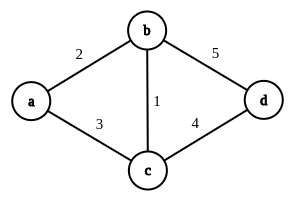
\includegraphics[width=0.6\linewidth, height=3.5cm,left]{7.png} 
\caption{Graph G}
\label{fig:subim1}
\end{subfigure}
\begin{subfigure}{0.5\textwidth}
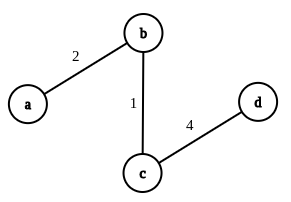
\includegraphics[width=0.6\linewidth, height=3.5cm,right]{6.png}
\caption{unique MST of G}
\label{fig:subim2}
\end{subfigure}
\begin{subfigure}{0.5\textwidth}
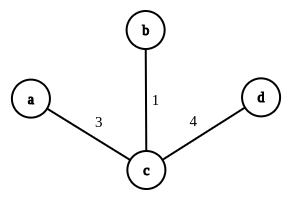
\includegraphics[width=0.6\linewidth, height=3.5cm,left]{5.png} 
\caption{second best MST of G}
\label{fig:subim3}
\end{subfigure}
\begin{subfigure}{0.5\textwidth}
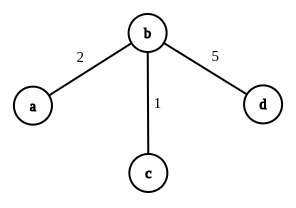
\includegraphics[width=0.6\linewidth, height=3.5cm,right]{4.png}
\caption{second best MST of G}
\label{fig:subim4}
\end{subfigure}
\caption{Counter-Example to prove non-uniqueness of second best MST of G}
\label{fig:image2}
\end{figure}\\\\
Hence claim Proved.
\newpage
\problem{Question 3: Continued}{5 + 5 + 5 + 5 points}
\subproblem{2}
\textbf{\underline{\textsc{Claim:}}}
There exists edges (u,v) $\in$ T and (x,y) $\notin$ T s.t. T - (u,v) $\cup$ (x,y) is a second best MST of G.\\\\
\textbf{\underline{\textsc{Proof:}}} \\\\Let T2 be a second best MST and T be MST. Let (u,v) $\in$ T - T2. Then, T2 $\cup$ (u,v) contains a cycle where one of the edges in the cycle is not in T (cycle property). Let this edge be (x,y). Then, we must have weight(x,y) $>$ weight(u,v), for otherwise, we could replace (u,v) in T by (x,y) to get a MST better than T. Now, we note that A = T2 - (x,y) $\cup$ (u,v) is also a spanning tree since (u,v) and (x,y) are in the same cycle. In addition, total-weight(A) $<$ total-weight(T2). So, A is a best MST. By the uniqueness of MST, we see that A = T.\\
Hence T = T2 - (x,y) $\cup$ (u,v), so T2 = T - (u,v) $\cup$ (x,y).Therefore T and T2 differ with only one edge, i.e. (u,v) replaced by (x,y). Hence Proved.\\\\
\subproblem{3}
\textbf{\underline{\textsc{Idea / Algorithm \& Analysis}}}\\\\
As $T{'}$ is a spanning tree meaning its a connected graph, every node can be reached from every other node. Hence using few heuristics to maintain max in the path between 2 vertices, we can iterate over al possible pair of vertices and find array max, where max[u,v] be an edge of maximum weight on the unique path between u and v in $T{'}$ for all u,v $\in$ V. We want to fill up the table max which has $|V|^{2}$ entries. For each vertex, the function DFS-NEW takes O(V) time. Hence overall the time complexity is O($|V|^{2}$).\\\\
\begin{algorithm}[H]
\SetAlgoLined
\KwData{$V,E \leftarrow $ {Vertex and edge sets of $T{'}$ from graph G respectively}}
\KwData{$W \leftarrow $ {weight set of edges}}
\KwResult{two-dimensional array max, containing edges}
\SetKwFunction{FRecurs}{DFSgraph-NEW(V,E,W)}%
\SetKwProg{Fn}{Function}{:}{}
\Fn(\tcc*[f]{algorithm as a recursive function}){\FRecurs}
{
    \For{each vertex u $\in$ V}
    {
        \For{each vertex v $\in$ V}
        {
            max[u,v] = NULL Edge;
        }
        DFS-NEW(V,E,W,max,u,u)\;
    }
Return max\;
}
\textbf{End Function}\\
\caption{finding max array in O($|V|^{2}$) time}
\end{algorithm}
\vspace{4mm}
\begin{algorithm}[H]
\SetAlgoLined
\SetKwFunction{FRecurs}{DFS-NEW(V,E,W,max,u,v)}%
\SetKwProg{Fn}{Function}{:}{}
\Fn(\tcc*[f]{algorithm as a recursive function}){\FRecurs}
{
\For{each vertex x, s.t. (v,x) $\in$ E}
{
    \If{(max[u,x]==NULL Edge) and (u!=x)}
    {   
        \uIf{(v==u) OR (weight(v,x) $>$ weight(max[u,v]))}
        {
             max[u,x] $\leftarrow$ (v,x)\;
        }
        \Else(\tcc*[f]{})
        {
            max[u,x] $\leftarrow$ max[u,v]\;
        }
        DFS-NEW(V,E,W,max,u,x)\;
    }
}
}
\textbf{End Function}\\
\caption{Recursive function DFS-NEW(V,E,W,max,u,v)}
\end{algorithm}
\vspace{4mm}
\newpage
\problem{Question 3: Continued}{5 + 5 + 5 + 5 points}
\subproblem{4}
\textbf{\underline{\textsc{Idea:}}}\\\\
From Sub-Problem 2, we know that we can replace one edge (u,v) in the MST, say T, by another edge (x,y) to get a second best MST, say T2. Note that if we replace (u,v) by (x,y), then $$totalweight(T2) = totalweight(T) - weight(u,v) + weight(x,y)$$
If we know which (x,y) to add to T2, then observe that (u,v) must be the max-weight edge in the path from x to y, which can be found by Sub-Problem 3. So, we get the following algorithm:\\\\
\textbf{\underline{\textsc{Algorithm:}}}\\\\
\begin{algorithm}[H]
\SetAlgoLined
\KwData{$V,E \leftarrow $ {Vertex and edge sets graph G respectively}}
T $\leftarrow$ MST of graph G\;
Find max-weight edges, 'max' array, as in Sub-Problem 3\;
Let max[x,y] denote the max-weight edge in the path from x to y in tree T, for all x,y $\in$ V\;
Find an edge (x,y) $\in$ E - T that minimizes (weight(x,y) - weight(max[x, y]))\;
Output T2 = (T - max[x,y]) $\cup$ (x,y)\;
\caption{Computes Second best MST in $O(|V|^{2}log|V|)$ time}
\end{algorithm}
\vspace{4mm}
\textbf{\underline{\textsc{Analysis:}}}\\\\
Line 1 takes $O(|E|log|V|)$ = $O(|V|^{2}log|V|)$ time as done in class using AVL tree. \\
Line 2,3 takes $O(|V|^{2})$ as done in Sub-Problem 3.\\
Line 4 also takes $O(|E|) = O(|V|^{2})$ as iteration through all edges takes place.\\
Hence time complexity of algorithm is $O(|V|^{2}log|V|)$.\\
\newpage
\problem{Question 4: Component Graph $G^{SCC}$}{3 + 3 points}
\\
\subproblem{1}
\textbf{\underline{\textsc{Claim:}}} $G^{SCC}$ is a DAG (Directed acyclic graph)\\\\
\textbf{\underline{\textsc{Proof (using contradiction):}}}\\\\
First, we observe, by definition that there cannot exist any strongly connected component of G which does not belong to $V^{'}$ --- (1)\\\\
Now let us assume $G^{SCC}$ to not be a DAG, meaning let's say $G^{SCC}$ has a cycle.\\
Then there exists strongly connected components $S_{1},S_{2}....S_{n} \in V^{'}$ which form a cycle in the component graph $G^{SCC}$.\\
Then taking all these components together we can get a bigger strongly connected component of G, which does not belong to $V^{'}$. This is contradiction to (1). Hence our assumption that $G^{SCC}$ is not a DAG is wrong. Hence we get that $G^{SCC}$ is indeed a DAG.\\ Hence proved.\\\\
\subproblem{2}
\textbf{\underline{\textsc{Claim:}}} $((G^{T})^{SCC})^{T} = G^{SCC}$\\\\
\textbf{\underline{\textsc{Proof:}}}\\\\
Let us try and prove this using fundamental basics of graphs.\\
Property 1: Two graphs are said to be equal if their edge and vertex sets are equal.\\
Property 2: Vertex sets of G and $G^{T}$ are equal.\\
Property 3: Strongly connected component (SCC) of G and $G^{T}$ are same.\\\\
Here first let us try and find relation between vertex sets of  $((G^{T})^{SCC})^{T}$ and $G^{SCC}$.\\
Using property 3, we can say vertex sets of $G^{SCC}$ and $(G^{T})^{SCC}$ are same. Which implies, using property 2, vertex sets of $(G^{T})^{SCC}$ and $((G^{T})^{SCC})^{T}$ are same, which further implies that vertex sets of $((G^{T})^{SCC})^{T}$ and $G^{SCC}$ are same.\\\\
Now let's find relation between edge sets of $((G^{T})^{SCC})^{T}$ and $G^{SCC}$.\\
Let $(v_{i},v_{j})$ be an edge in $((G^{T})^{SCC})^{T}$. Then $(v_{j},v_{i})$ will be an edge in $(G^{T})^{SCC}$. Now there exists $a \in C_{j}$ (the SCC denoted by $v_{j}$)  and $b \in C_{i}$ (similarly for i), s.t. (a,b) is an edge in $G^{T}$. Therefore (b,a) is an edge in G. Since vertex sets haven't been altered in any sense, property 3 holds, and we get that $(v_{i},v_{j})$ is an edge in $G^{SCC}$. Hence using this iteratively over the entire set of edges in $((G^{T})^{SCC})^{T}$,we get that all of those edges in $((G^{T})^{SCC})^{T}$ also belong in $G^{SCC}$. For the other direction, we can similarly prove that all edges in $G^{SCC}$ also belong in $((G^{T})^{SCC})^{T}$. Hence we get the edge sets of $((G^{T})^{SCC})^{T}$ and $G^{SCC}$ equal.\\\\
Hence our claim $((G^{T})^{SCC})^{T} = G^{SCC}$ is true using property 1.\\
Hence proved.\\
\newpage
\problem{Question 5: Euler Tour}{6 + 5 points}
\subproblem{1}
\textbf{\underline{\textsc{Claim:}}} A directed graph G=(V,E) has an Euler Tour iff indeg(v)=outdeg(v) for each v $\in$ V.\\\\
\textbf{\underline{\textsc{Proof:}}}\\\\
Let us first prove that if G has an Euler Tour then indeg(v)=outdeg(v) for each v $\in$ V.\\ G has an euler tour, T, meaning that T is a cycle. If T is a simple cycle then$$ indeg(v) = outdeg(v) = 1,\forall v \in V$$ so the claim is true.\\
If T is not a simple cycle then it will have one or more simple cycles. After we remove (delete edges of) one simple cycle from T (and G), then T will still remain Euler tour. Keep removing (deleting edges of) the simple cycles from T (and G) until no edges are left. Now at this point, indeg(v) = outdeg(v) = 0, $\forall v \in V$. Also we observe that when removing a cycle, an in-edge and out-edge of the vertices on the cycle are removed, and hence after a cycle deletion, the in-degree and out-degree of a vertex on the cycle decrease by exactly 1. So the conclusion we come to is that before any deletions took place, indeg(v)=outdeg(v) all vertices v $\in$ V.\\\\
Here let us claim something which will help us with our next part proof. \\
\underline{Sub-Claim:} for any vertex v with indeg(v)=outdeg(v), there must be a path starting from v that comes back to v.\\
\underline{Proof:} For any vertex v, there must be a cycle that contains v. Start from v, and chose any outgoing edge of v, say (v, u). Since indeg(u) = outdeg(u) we can pick some outgoing edge of u and continue visiting edges. Each time we pick an edge, we can remove it from further consideration. At each vertex other than v, at the time we visit an entering edge, there must be an outgoing edge left unvisited, since indeg = outdeg for all vertices. The only vertex for which there may not be an unvisited outgoing edge is v, because we started the cycle by visiting one of v’s outgoing edges. Since there’s always a leaving edge we can visit for any vertex other than v, eventually the cycle must return to v, thus proving the sub-claim.\\\\
Now let us prove that if indeg(v)=outdeg(v) for all v $\in$ V then G has an Euler tour.\\
Now we pick a random vertex v, and find a cycle T that comes back to v (as proved above). Delete all the edges of T from G. Each vertex in the updated G has indeg(v)=outdeg(v), so we pick a vertex $v^{'}$ on T that has some edges going out and coming into it. We repeat our process.\\
Overall we find a cycle T, then another cycle $T^{'}$ that has (at least) a common vertex with T, and so on. We can build a big cycle that goes around T jumps in $T^{'}$ and goes around $T^{'}$ and then comes back to T and finishes in T.\\\\
Hence we proved our claim  both ways. Hence Proved.\\\\ Hence a directed graph G=(V,E) has an Euler Tour iff indeg(v)=outdeg(v) for each v $\in$ V.\\

\newpage
\problem{Question 5: Continued}{6 + 5 points}
\subproblem{2}
\underline{\textsc{Idea / Algorithm}}\\\\
\begin{algorithm}[H]
\SetAlgoLined
\KwData{$V,E \leftarrow $ {Vertex and edge sets graph G respectively}}
First we can simply check whether indeg(v)=outdeg(v) for all v $\in$ V\; if false then return "Euler tour does not exist"\;
else we continue and find the Euler tour\;
let us define DFSNEW as the modified DFS so that we store, for each edge that we traverse,
a pointer to the corresponding edge in the adjacency list of G\;
Pick a vertex v\;
do DFSNEW on v until we come across a back edge that links back to v\;
Once we find this cycle, traverse all edges of the cycle, and delete the corresponding edges in the adjacency list of G\;
repeat (from line 5) until no edges remain in G\;
\caption{Computes Euler Tour of Graph}
\end{algorithm}
\vspace{4mm}
\textbf{\underline{\textsc{Analysis:}}}\\\\
lines 1-3 take O($|E|$) time\\
DFSNEW in line 4 will help the deletion of edges in line 7, by making the deletion to be done in constant time, as no need to search for edges in G because of use of pointers.\\
lines 4-8, DFSNEW, also takes O($|E|$) time as each edge has to be looked at once and then it is deleted.\\\\
Hence time complexity to find out the Euler Tour of G is O($|E|$) time or linear time.\\
\\
\\
\item[4.15]Show that the problem of determining whether a CFG generates all strings in 1* is decidable. In other words, show that \{\angles{G} $|$ $G$ is a CFG over $\{0, 1\}$ and $1^* \subset L(G)$\} is a decidable language. 
\\
\textbf{Solution:} Let $f$ be a computable function. Construct a decider $D$:
\\
$D$ = ``On input \angles{G} where $G$ is a CFG:
\begin{enumerate}
\itemsep0em
\item[1.]Convert $G$ into an equivalent CFG $C$ in Chomsky Normal Form.
\item[2.]Let $p$ be the pumping length of $C$.
\item[3.]Repeat $0 \le i \le p + p!$:
\begin{enumerate}
\item[a.]Check whether $1^i \in L(C)$.
\item[b.]If not, $reject$ \angles{G}.
\end{enumerate}
\item[4.]$Accept$ \angles{G}.
\end{enumerate}
We can check $1^i \in L(C)$ using the Cocke-Younger-Kasami (CYK) algorithm for CFGs, which has a running time of $\Theta(n^3 |G|)$. Therefore, the loop has a running time of $\Theta(pn^3 |G|)$. Since Steps 1, 2, 3, and 4 take finite time, this language is decidable.
\\
\end{document} 
